\chapter{Research Methodology}
\label{ch:research-methodology}

\section{Research Model}
\label{sec:research-model}
	\begin{figure}[h]
		\centering
		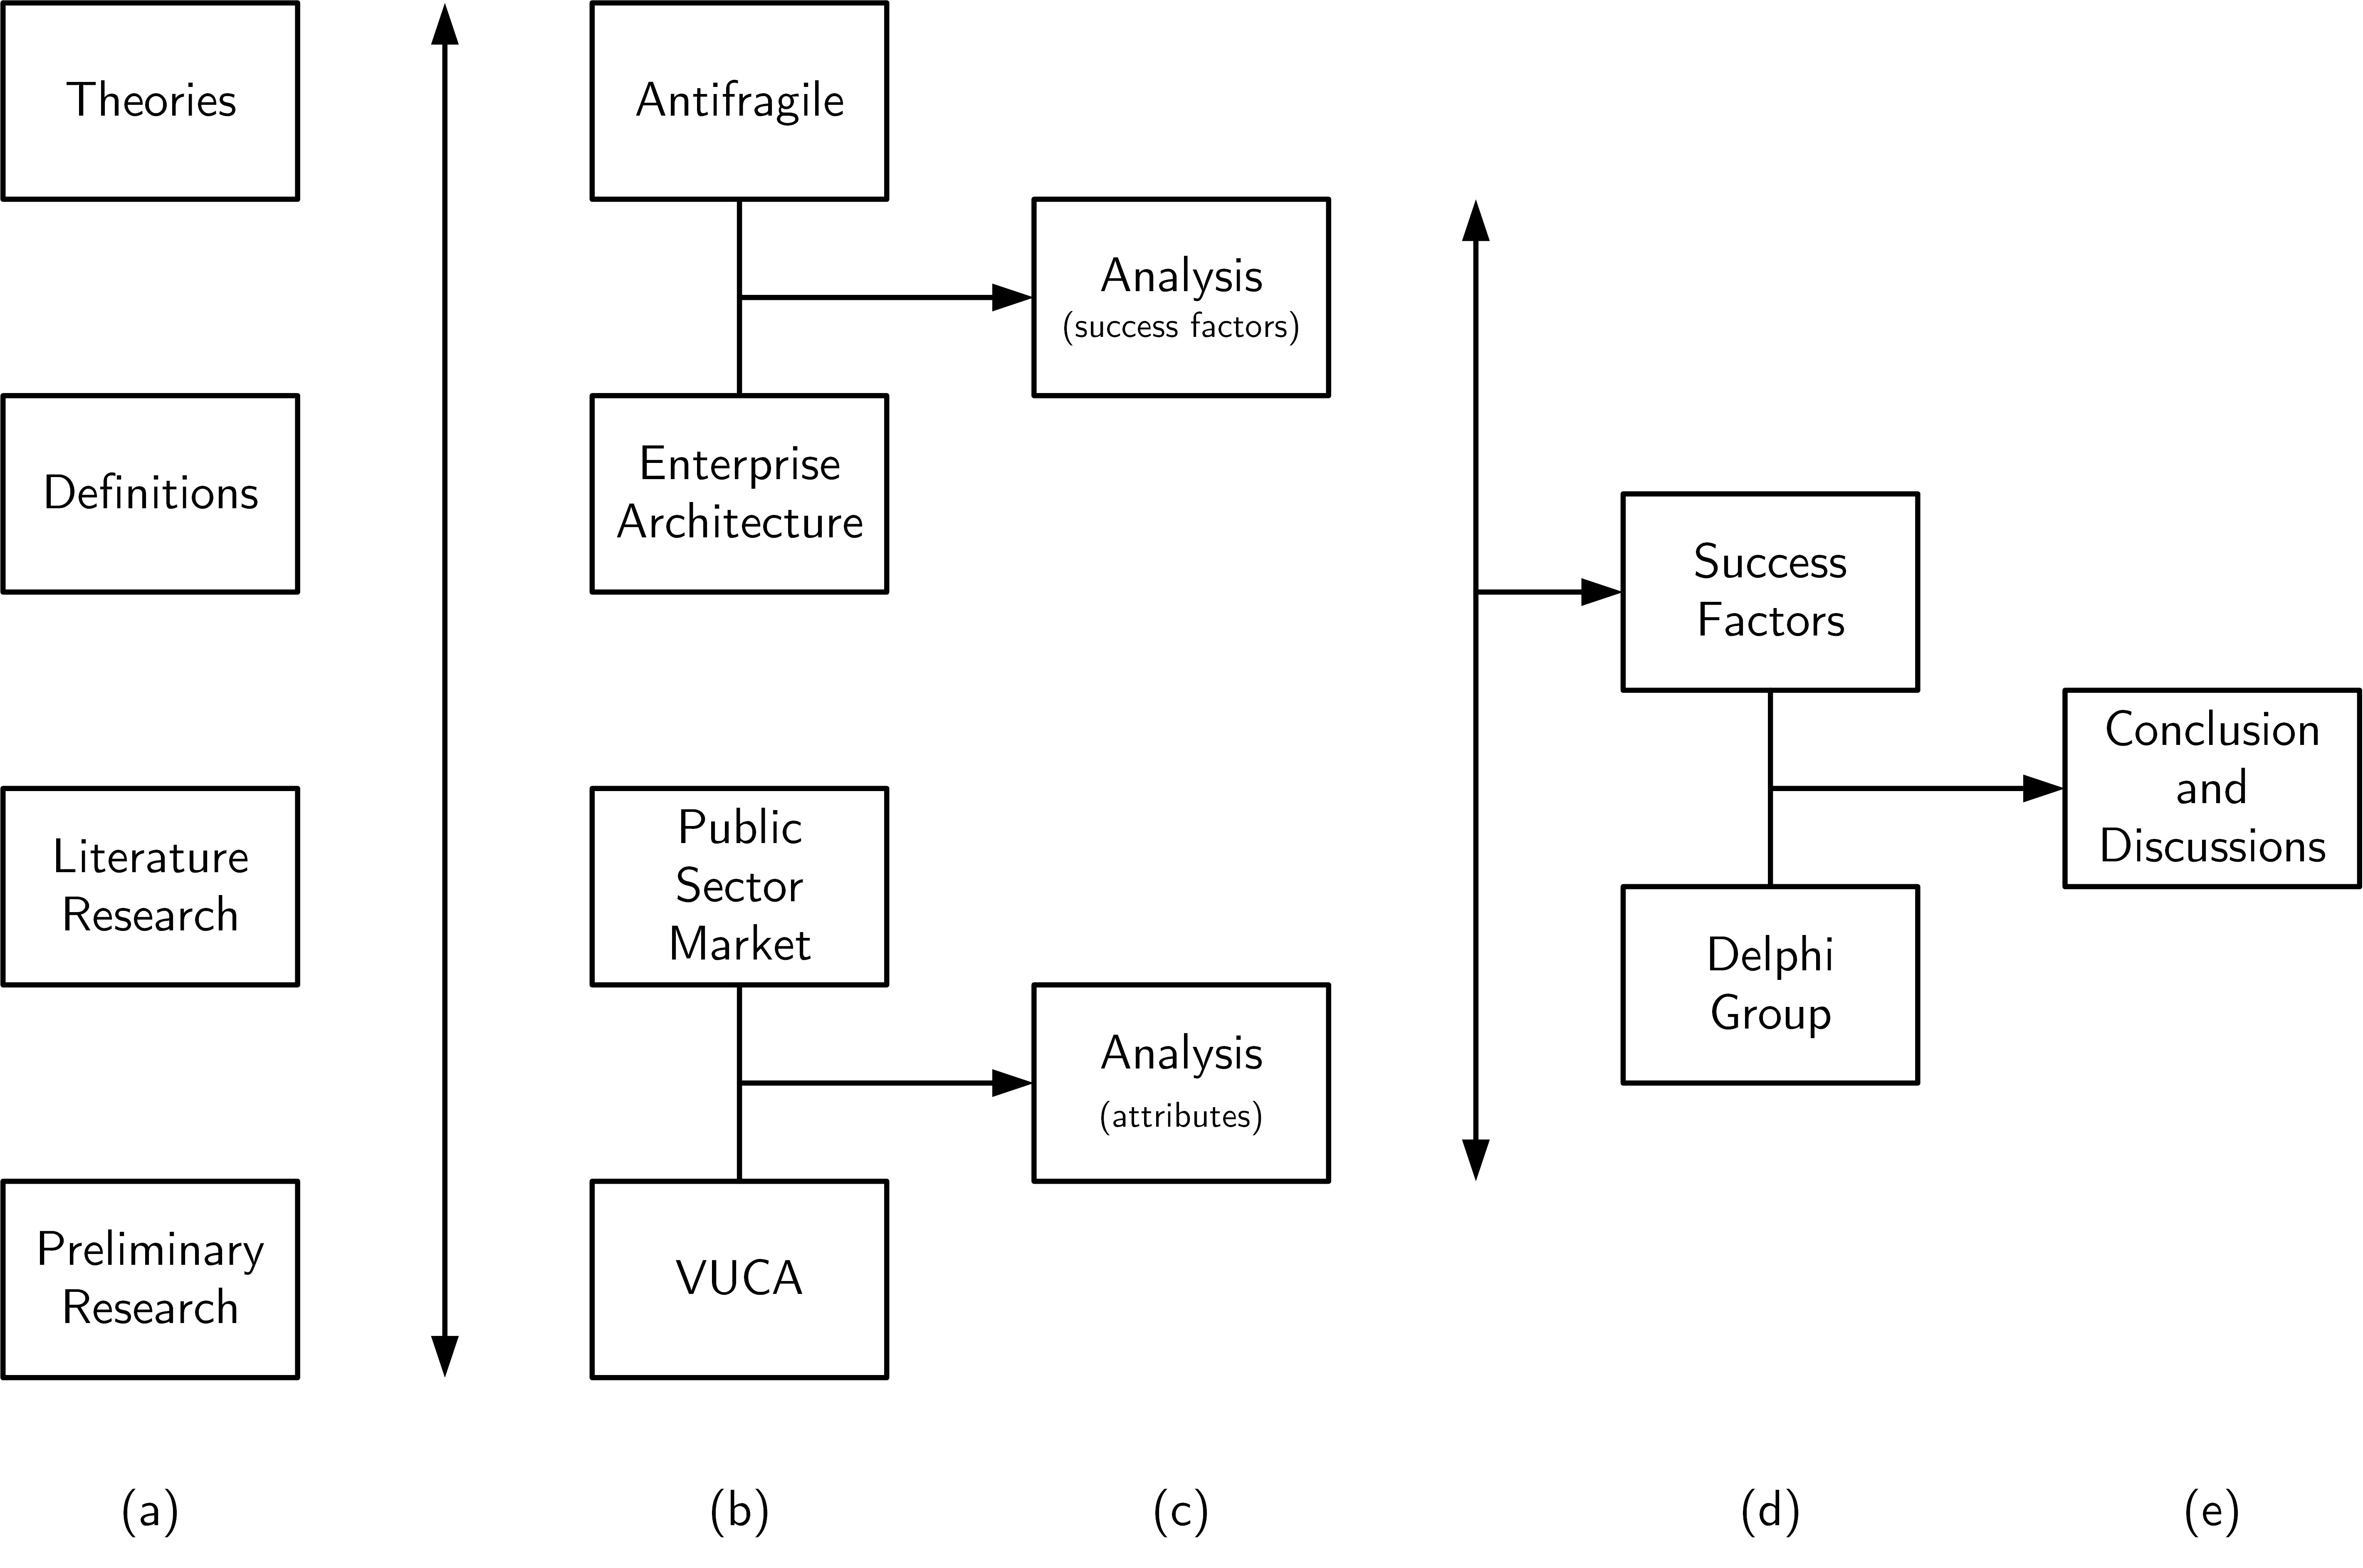
\includegraphics[width=12cm]{images/research-model.png}
		\caption[Research Model]{Research Model}
		\label{fig:research-model}
	\end{figure}

\section{Delphi Group}
For the Delphi Group participants see appendix~\ref{app:delphigroupparticipants} \\%

What about the sample size? Normally Delphi is about 100+. What about this research. How large should the sample size be for a qualitative result?

\section{Quality of the Research (old example text)}
\label{sec:quality-of-the-research}
The research was qualitative. The information is based on qualitative information gathered by the researcher
from employees of the organisation. However, with the research approach and transparency, the research can
be validated, can be repeated, so it is reliable and reducible. With the use of managerial models and methods
like Lean, Value Stream Mapping with supporting tools like NEN-ISO/IEC 25011 and ServQual got a nonbiased
result.\\
\begin{itemize}
	\item{\textbf{The validity} of the research is dependent on the right use of the right models and the right methods. The researcher conducted research on which models, frameworks and tools to use. The results and the rationales around the choice of theories, models, frameworks and tools are stated in chapter 4. The sources used for determining the theories, models, frameworks and tools are from scientific and expert sources.}
	\item{\textbf{The reliability} is about the influence of possible errors. For the research, the researcher used methods like triangulation, and sources from scientific reports and expert literature. The number of interviews was too small for the right statistical outcome. To enlarge the reliability of the interviews, the researcher used the same framework of themes for his semi-structured interviews. The transcriptions are placed in the appendixes for transparency. The information gathered with the interviewees is compared with the other interviewees.}
	\item{\textbf{The repeatability} is about getting the same results when the research is conducted again. The researcher uses his research design and research approach, as stated. All the steps taken are put into the research design. If this research design is followed, the same results should follow.}
	\item{\textbf{The reducibility} is about the outcome of the research can be deducted step by step. By using the research model, and the structure of the thesis, every step is reducible.}
\end{itemize}

\begin{itemize}
	\item{Think about Replication}
	\item{Recker types}
	\item{OpenScience}
	\item{Howto falsify?}
	\item{Rigourness}
\end{itemize}


\section{Used research tooling}

\LaTeX\ with the KOMA-Script Report template\\
TeXstudio\footnote{https://www.texstudio.org/}\\
TeX Live\footnote{https://tug.org/texlive/}\\
Dropbox\footnote{https://www.dropbox.com/}\\
GitHub\footnote{https://github.com/} (2 repositories) \\
	Master Thesis Repository\footnote{https://github.com/JRBliekendaal/master-thesis}\\
	Master Thesis Administration Repository\footnote{https://github.com/JRBliekendaal/master-thesis-administration}\\
GitHub Desktop\footnote{https://desktop.github.com/}\\
JabRef\footnote{https://www.jabref.org/} as a reference manager including integration with web browsers\\
PaperPanda\footnote{https://paperpanda.app/} for finding hard to find resources\\
Grammarly\footnote{https://www.grammarly.com/}

Microsoft Excel\\
Microsoft Powerpoint\\
Microsoft Visio\\
Sparx Enterprise Architect\\


Researchgate\\
Web of Science\\
Google Scholar\\
Meetingwizard\footnote{https://www.meetingwizard.nl/}\\


Hardware\\
Dell Windows PC with Windows 10\\
Amazon Kindle Oasis\\

leuchtturm1917 notebooks\\
